% 第2章：依课件2.1--2.8顺序整理；标注课件例题、参考书补充及必要核对说明。
\chapter{物理层}

\noindent\textbf{本章要解决的问题。} 上一章把一条链路看成能够发送比特的通道，本章打开这条通道：0和1怎样变成线路上的信号，接收方怎样认出它们，什么限制传输速率，多路通信怎样共用一条线路。物理层向数据链路层提供比特流传输能力；至于这些比特组成什么帧、属于哪个地址，将在下一章讨论。

\noindent\textbf{阅读提示。} 按课件的八节顺序学习。先把数据、信号、码元、比特率和波特率分清，再使用容量公式；看到波形时先找时间边界，看到公式时先核对单位。本章的“学习补充”和“自拟例”用于解释必要基础，不作为课件原题或课堂原话。

\section{物理层基本功能}
\subsection{从比特到信号：物理层做什么}
计算机内部保存的比特只有0和1，但一根导线不会直接运输抽象的数字。发送端必须选择一种物理表示，例如用两种电压、两种光脉冲状态或两种载波相位表示数据；接收端观察信号，并按相同约定恢复比特。这组约定和实现就是物理层研究的内容。

\textbf{物理层的基本功能}是在连接结点的物理介质上实现比特流传输。具体要约定比特编码、数据率、比特同步、接口特性和传输模式。例如，若双方约定每个比特持续$1\,\mu\mathrm{s}$，接收方就要知道该在什么时刻观察电平；只有双方采用相同规则，接收到的波形才会被解释成相同的0和1。

\textbf{学习补充：介质与层次。} 铜线、光纤和自由空间提供信号经过的物理通路；物理层规定如何利用这条通路传输比特。介质本身不能决定“这一电压代表0还是1”，因此在网络体系结构中，介质位于物理层之下。不要把网线本身当成物理层协议。

\annotationarea[4]

\subsection{DTE、DCE与接口的四类特性}
\textbf{数据终端设备（DTE，Data Terminal Equipment）}是产生或使用数据的设备，例如计算机终端。\textbf{数据电路终结设备（DCE，Data Circuit-terminating Equipment）}位于DTE与传输线路之间，负责使数据适合线路传输，例如调制解调器（Modem）。课件还以网络接口卡（NIC，Network Interface Card）举例；实际网卡常同时承担物理层和数据链路层功能，不能据此把整块网卡限定为物理层设备。

接口是两部分连接并交换信号的边界。物理层协议必须回答“能否插上、信号合不合要求、每根线是什么意思、何时执行什么操作”四类问题：
\begin{center}
\begin{tabularx}{0.97\textwidth}{l X X}
\toprule
特性 & 规定什么 & 用来辨别的例子\\
\midrule
机械特性 & 接线器形状、尺寸、引脚数量与排列、固定方式 & 插头形状和引脚位置\\
电气特性 & 电压范围等电路要求及相关传输限制 & 某信号线允许的电压范围\\
功能特性 & 各线路的作用及电平的含义 & 某引脚是时钟线；有效电平表示发送请求\\
过程（规程）特性 & 功能事件的先后顺序和时序关系 & 先请求发送，再等待允许，随后传送数据\\
\bottomrule
\end{tabularx}
\end{center}
在DTE与DCE之间，除了串行比特流还可能交换控制信息；在DCE与介质之间，约定信号线和控制线如何承载信号。课件示意图用用户设施与通信设施标出这两个接口边界。
\textbf{辨别方法。} “允许多大电压”问电气条件；“这个电平表示什么”问功能含义；“先出现哪个事件”问过程。介质访问控制（MAC）地址属于数据链路层的标识，不属于这四类物理接口特性。

\begin{quote}\small 来源：课件\texttt{Chapter2-物理层.pdf}，PDF第3--7页（显示页3--7）；教材§2.2.2，PDF第55页／印刷第44页；介质与层次关系见教材§2.4，PDF第59--60页／印刷第48--49页。\end{quote}
\annotationarea[4]

\section{数据通信基础}
\subsection{数据、信号与通信系统}
\textbf{数据}是用于传送信息的实体，例如用二进制表示的文字、图像或语音样本。\textbf{信号}是数据的电气或电磁表示，例如随时间变化的电压、光强或无线电波。数据讲的是“要表达什么”，信号讲的是“用什么物理变化来表达”。同一比特串可以采用不同信号表示。

模拟量取值连续，数字量取值离散。模拟数据的例子是原始声音的连续变化；数字数据的例子是编码后的比特串。数字数据既可以用数字信号传输，也可以控制连续载波来传输，因而\textbf{“传的是数字数据”不等于“线路上一定是方波”}。后文的PCM与调制分别展示这两种变换。

\textbf{频带（频谱）}是信号占有的频率范围；\textbf{带宽}是有效频带的宽度，常以Hz表示。带宽窄表示可用频率范围窄，不能仅由这个词推断数据率的数值；后文公式会说明特定信道模型下的关系。

课件用正弦信号$y(t)=A\sin(\omega t+\theta)$说明信号可随时间变化；$A$是振幅，$\omega$是角频率（单位rad/s），$\theta$是相位。角频率与频率$f$的关系是$\omega=2\pi f$，其中$f$以Hz计量。本章后面介绍载波调制时会再次使用这些量。

按课件模型，一次单向传输经过如下环节：
\[
\text{信源}\longrightarrow\text{发送设备}\longrightarrow\text{信道}
\longrightarrow\text{接收设备}\longrightarrow\text{信宿}.
\]
信源产生数据；发送设备进行编码或调制；信道承载信号；接收设备作相应反变换；信宿使用恢复出的数据。\textbf{噪声}是干扰信号的成分，可能来自环境，也可能来自设备。它可能使接收方把本来表示1的信号误判为0。
\annotationarea[4]

\subsection{码元、比特率、波特率与带宽}\label{sec:physical-rates}
\textbf{码元}是在一个固定时长内用来表示符号的一段信号波形，也可称信号基本单元。其时长记为$T_s$；每秒发送的码元数是\textbf{码元速率或波特率}$R_B=1/T_s$，单位Baud。\textbf{比特率}$R_b$表示每秒传送的比特数，单位bit/s或b/s。

\textbf{为什么一个码元不一定只代表一比特？} 若只有两种可区分状态，可以分别代表0、1；若有四种状态，可以分别代表00、01、10、11，一次选择就传出两比特。一般地，$k$比特共有$2^k$种组合。因此，当$M=2^k$种码元状态都用于等长二进制映射时，每码元携带
\[
 k=\log_2M\quad\text{bit},\qquad R_b=R_B\log_2M.
\]
这里$\log_2M$的意思是“2的几次方等于$M$”：$\log_2 4=2$、$\log_2 8=3$、$\log_2 16=4$。本章计算题中的$M$通常是2的整数次幂。增加状态数可以增加每码元的信息量，但接收方需要更清楚地区分这些状态。

\textbf{自拟例：} 信号每秒发送$1000$个码元，每码元从$16$种状态中选择一种。先求每码元信息量$\log_2 16=4$ bit，再算$R_b=1000\times4=4000$ bit/s。反过来，若比特率为$64$ kb/s、每码元有4种状态，则$R_B=64000/2=32000$ Baud。波特率与比特率只有在一比特对应一码元时才数值相等。

\textbf{频率}表示每秒振荡的周期数，单位赫兹（Hz）；\textbf{频率带宽}$B$表示信道能通过的频率区间宽度，单位也是Hz。例如$3.5$--$3.9$ MHz的区间宽度为$0.4$ MHz。网络性能中也常把最大数据传输速率称作“带宽”，单位是b/s；本章容量公式中的$B$始终是\textbf{频率带宽}。

\begin{center}
\begin{tabularx}{0.97\textwidth}{l l X}
\toprule
量 & 单位 & 回答的问题\\
\midrule
频率带宽$B$ & Hz & 能容纳多宽的频率范围？\\
波特率$R_B$ & Baud & 每秒发送多少个码元？\\
比特率$R_b$ & b/s & 每秒传送多少个比特？\\
\bottomrule
\end{tabularx}
\end{center}
\textbf{易错点。} 信号沿线路传播的速度用m/s计量，与每秒送入线路多少比特的比特率不同。二进制数据也可以映射为多进制码元；“数据是二进制”不自动推出$M=2$，需看题目是否限定只有两种信号状态。
\annotationarea[4]

\subsection{通信方向与串行、并行：两组不同的分类}
\textbf{单工}只允许一个方向传输，例如广播接收；\textbf{半双工}允许双方发送，但需要轮流，例如按下发送键才能讲话的对讲机；\textbf{全双工}允许双方同时发送和接收，例如正常的双向电话交谈。这组分类回答的是“两个方向是否能够同时工作”。全双工需要两方向可同时使用的传输能力，不等于必须有两根独立网线。

\textbf{串行传输}按顺序逐比特发送；\textbf{并行传输}用多条通道同时发送多个比特。这组分类回答的是“同一方向的一组比特怎样送出”。例如发送字节10110010，串行方式依约定次序逐个发送；8路并行方式可在同一传送时刻分别送出8位。为远距离链路铺设多条线路并保持各路同步成本较高，网络通信通常采用串行方式。串行并不意味着只能单工，也不意味着所有串行系统都比并行系统慢。
\annotationarea[4]

\subsection{为什么需要时钟同步}
发送端把时间分成一个个比特或码元区间，接收端必须知道每个区间从哪里开始，并在合适的位置取样。若接收端时钟略快或略慢，取样位置会逐渐漂移，最后可能把相邻比特认错；长串相同电平又无法直接显示比特边界。

\textbf{异步通信}的典型方式是逐字符传输。双方各有时钟，但每个字符开始时利用起始位重新对齐。

课件给出的字符通常含5--8个数据位，起始位标记字符开始；校验位（parity bit）可选，用于检查部分传输差错；停止位占1或2个比特时间并回到逻辑1的空闲状态。发送端和接收端在一个字符内按约定速率取样，字符之间可以留不等长空闲时间。课件图中的空闲逻辑值为1，起始位为0，因此接收端检测到从1到0的跳变后开始计时。

图\ref{fig:async-character}展示一个字符的格式。其中，Start bit为起始位，Data bits为数据位，P bit为可选校验位，Stop element为停止位。接收方从起始位边沿开始计时，在约定的位中心取样后续数据。

\begin{figure}[H]
 \centering
 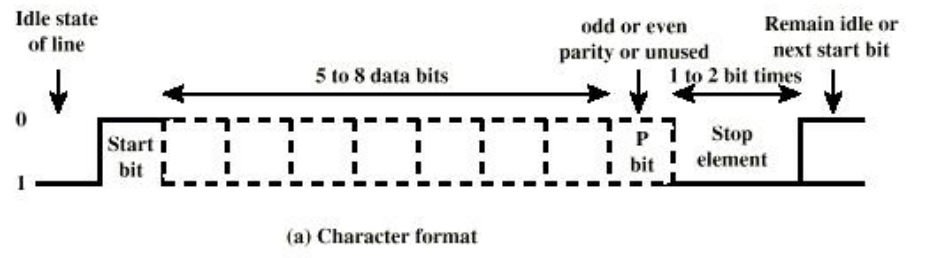
\includegraphics[width=0.86\textwidth]{ch02-async-character.png}
 \caption{异步通信的字符格式。来源：\texttt{Chapter2-物理层.pdf}，PDF第12页（显示页12），局部截取。图中0、1是逻辑状态标注，不能只凭波形画在上方或下方判断其数值。}
 \label{fig:async-character}
\end{figure}

\textbf{计算例：} 若采用1位起始位、8位数据位、1位停止位且不加校验位发送一个字符，总计$1+8+1=10$位；有效数据占$8/10=80\%$，起止附加位占$2/10=20\%$。若再加校验位或使用2位停止位，应把它们计入总位数。

课件列出的优点是实现简单、成本低；代价是每个字符需增加2或3个附加位，课件以约20\%开销概括。它适合短距离、低速率、字符间隔较大的场景，例如键盘输入。实际开销比例取决于数据位、校验位、停止位的配置。

\textbf{同步通信}通常连续传送较大数据块。双方需维持一致的时序，可以使用单独时钟线（适合短距离，且时钟线也可能受损），也可以把时序线索嵌入数据信号或载波中。后文Manchester编码每比特中间都有一次跳变，就可提供时序线索。同步方式减少逐字符起止位开销，但仍可能有同步、组帧或其他开销，不能理解为没有任何附加信息。
\annotationarea[4]

\subsection{模拟通信与数字通信}
课件按信道中传输的信号区分模拟通信与数字通信：传输模拟信号的是模拟通信，传输数字信号的是数字通信。这里判断的是\textbf{信道上实际传输的信号}，不是只看信源原始数据是语音、图像还是比特。例如，模拟语音经过PCM后成为数字信号，可以进入数字通信系统；数字比特也可控制载波，产生连续变化的已调信号。此处的“模拟/数字信号”与“模拟/数字数据”需分开判断。
\annotationarea[4]

\subsection{模拟数据数字化：PCM的三个步骤}
\textbf{脉冲编码调制（PCM）}把模拟数据转换为数字表示。虽然名称中有“调制”，这里讨论的是模拟信源的数字化；它不同于后文用数字数据改变载波的数字调制。
\begin{enumerate}
 \item \textbf{采样：} 在一系列离散时刻读出原信号幅值，使时间离散；幅值此时还可连续取值。
 \item \textbf{量化：} 把幅值映射为预设的有限量化等级，使取值离散。原幅值与代表值之间存在量化误差。
\item \textbf{编码：} 用二进制码表示量化等级。若有$N$级，固定长度编码至少需要$k=\lceil\log_2N\rceil$ bit；若$N=2^k$则正好用$k$ bit。课件简写为$\log_2N$位，对$N$为2的幂次时成立；其他$N$取固定码长时要向上取整。
\end{enumerate}
图\ref{fig:pcm-process}先显示连续波形，再给出3.2、3.9等采样值；量化后成为3、4等等级；最后分别编码为011、100等。图中的脉冲幅度调制（PAM，Pulse Amplitude Modulation）脉冲行表示采样时刻的幅值，下一行体现量化，不可把两行混成同一步。

\begin{figure}[H]
 \centering
 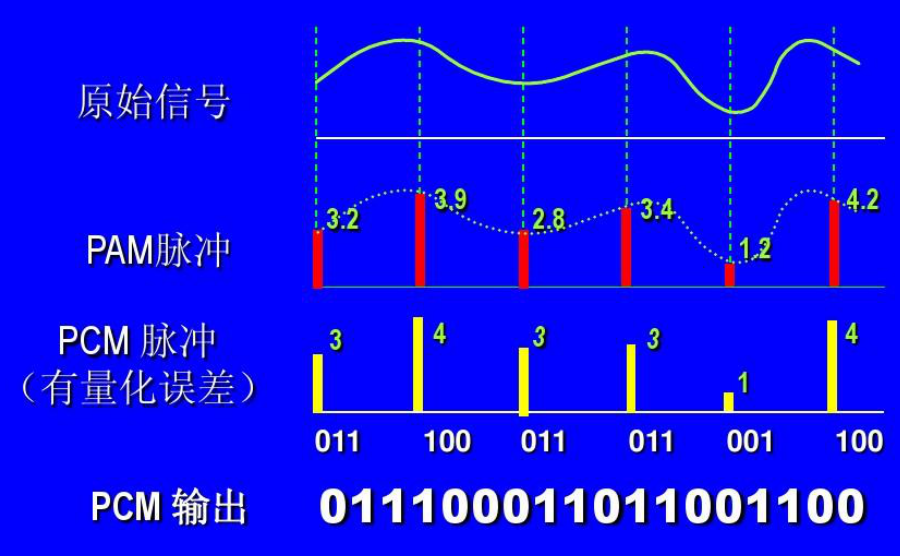
\includegraphics[width=0.78\textwidth]{ch02-pcm-process.png}
 \caption{PCM从连续波形到采样、量化、二进制码的过程。来源：\texttt{Chapter2-物理层.pdf}，PDF第19页（显示页19），局部截取。}
 \label{fig:pcm-process}
\end{figure}

\textbf{课件例题（PDF第19页／显示页19）：} 图中六个采样值依次为3.2、3.9、2.8、3.4、1.2、4.2。按课件的量化格点，它们分别量化为3、4、3、3、1、4；每个等级用3位二进制表示，逐个查码为
\[
3\mapsto011,\quad4\mapsto100,\quad3\mapsto011,\quad3\mapsto011,\quad1\mapsto001,\quad4\mapsto100.
\]
因此输出比特流为$011\ 100\ 011\ 011\ 001\ 100$，去掉分组空格为\texttt{011100011011001100}。量化后的等级可恢复，原采样幅值（例如3.2）不能由码字精确恢复。
\annotationarea[4]

\textbf{参考书补充：采样条件与PCM码率。} 采样过慢时，原来的快速变化可能被误认成较慢的变化，这称为\emph{混叠}。对最高频率为$f_{\max}$的理想带限信号，为避免混叠并重建原信号，通常取$f_s>2f_{\max}$。教材用“不得低于两倍”概括这个条件；$2f_{\max}$是理论边界，等号不能对任意恰好位于带边的信号无条件保证重建。实际设计需要留余量，并先限制输入频带。采样定理不消除随后量化造成的误差。这里限制的是\emph{采样原模拟信号的频率}，不要与后文的无码间串扰码元速率限制混用。若每秒采样$f_s$次、每样本编码$k$ bit，不考虑其他开销，则PCM比特率
\[
 R_{\mathrm{PCM}}=f_sk.
\]
\textbf{自拟例：} 将最高频率3 kHz的带限信号每秒采样8000次，满足$8000>2\times3000$，采用256级量化，则$k=\log_2 256=8$，输出码率$8000\times8=64000$ bit/s，即64 kb/s。这只是数字化后的数据率，不表示一条3 kHz模拟信道可无条件以64 kb/s传输。
\annotationarea[4]

\subsection{扩频：把信息展开到更宽频带}
\textbf{扩频}使承载信息的信号占用比原始数据所需更宽的频带。课件说明可用于模拟或数字数据，并以扩展频带使通信不易被窃听作为用途说明；这不等于加密或保密保证。课件介绍两类：\textbf{跳频}按双方知道的序列在一组载波频率间跳换；\textbf{直接序列扩频}用较长的码片序列表示原来的一比特。接收方依据同样的序列恢复信息。这里“一个信息比特对应多个码片”的想法，也会用于2.5节的码分复用。

课件英文将跳频写作“Frequency hoping”，应为“Frequency hopping”（跳频）。发送端与接收端按共享序列切换频率。

\textbf{学习补充：} 扩频可改善对窄带干扰的抵抗，并可支持不同用户在同一频带工作。它需要相应的同步、编码和接收处理；仅扩展频带不能替代加密。课件还将跳频思想与好莱坞演员Hedy Lamarr联系起来，属于历史备注。

\begin{quote}\small 来源：课件PDF第8--20页（显示页8--20）；教材§2.1.1，PDF第41--42页／印刷第30--31页，§2.1.3的PCM说明，PDF第45页／印刷第34页。对数、PCM码率和80\%效率例是按来源规则补出的基础说明或自拟计算。\end{quote}
\annotationarea[4]

\section{物理介质}
\subsection{导引型介质：信号沿指定通路传播}
导引型介质把信号限制在指定的物理通路中。课件列出架空明线、双绞线、同轴电缆和光纤。

\textbf{架空明线}是架设在空中的裸导线，容易受天气和外界电磁干扰，课件指出其带宽有限。

\textbf{双绞线}由两根绝缘导线相互绞合而成，主要用于基带传输。屏蔽双绞线简称STP（Shielded Twisted Pair），非屏蔽双绞线简称UTP（Unshielded Twisted Pair）。课件给出的UTP类别、频率带宽和典型应用如下：
\begin{center}
\small
\begin{tabularx}{0.97\textwidth}{c c X}
\toprule
类别 & 频率带宽 & 课件列出的典型应用\\
\midrule
3类 & 16 MHz & 低速网络、电话网络\\
4类 & 20 MHz & 10BASE-T以太网\\
5类 & 100 MHz & 10BASE-T以太网、100BASE-T快速以太网\\
超5类（5E） & 100 MHz & 100BASE-T快速以太网、1000BASE-T吉比特以太网\\
6类 & 250 MHz & 1000BASE-T吉比特以太网、ATM网络\\
\bottomrule
\end{tabularx}
\end{center}
表中MHz是线缆频率带宽，不是网络数据率；例如100 MHz不能直接读成100 Mb/s。实际链路速率还取决于接口标准、编码方式、线缆长度等条件。
表中10BASE-T、100BASE-T和1000BASE-T表示相应速率等级的双绞线以太网，后缀T表示双绞线介质；ATM是异步传递模式（Asynchronous Transfer Mode）。

\textbf{同轴电缆}由内导体、绝缘层、外导体屏蔽层和保护套组成，屏蔽结构提高抗干扰能力。课件主要以频带传输举例；\textbf{参考书补充}说明同轴也可用于基带传输，例如早期基带以太网采用50$\,\Omega$电缆，有线电视常用75$\,\Omega$电缆。因此“同轴”描述介质结构，不能独自决定采用基带还是频带技术。

\textbf{光纤}用光导纤维约束并传输光信号。用光线模型理解，纤芯折射率高于包层；当光从纤芯射向包层的入射角满足条件时，光不会折射到包层外，而是在界面反射回纤芯，这称为\textbf{全反射}。光纤不以金属导体中的电流承载数据，因而抗电磁干扰能力强、传输损耗较小、容量潜力大。

光纤分\textbf{多模}和\textbf{单模}。多模允许多种传播模式，传播路径/到达时间的差别会使短光脉冲展宽，限制距离和速率；单模只允许一种传播模式，避免多模间的到达时间差，更适合长距离高速传输。这里的“模”是传播方式，并非信号幅度的“模拟”或数据的“数字”，也不等于“只传一条信息”。教材用直线与反射作示意，本节只用它建立直觉，不把单模定义为光从不受波导约束。

课件在本节点出各介质类别和光纤的基本原理；UTP参数表按课件逐项列出，双绞线、同轴和光纤结构细节则由教材补充。
\annotationarea[4]

\subsection{非导引型介质：自由空间中的传播}
非导引型介质在自由空间中传播电磁波。课件按频率范围列出无线电、红外线、可见光和紫外线等频段及其应用。下表转录课件第24页的频率范围与典型应用；频率范围采用课件给出的近似值。
\begin{center}
\small
\begin{tabularx}{0.97\textwidth}{l l X}
\toprule
频率范围 & 名称 & 课件列出的典型应用\\
\midrule
3--30 Hz & 极低频（ELF） & 远程导航、水下通信\\
30--300 Hz & 超低频（SLF） & 水下通信\\
300--3000 Hz & 特低频（ULF） & 远程导航\\
3--30 kHz & 甚低频（VLF） & 远程导航、水下通信、声纳\\
30--300 kHz & 低频（LF） & 导航、水下通信、无线电信标\\
300--3000 kHz & 中频（MF） & 广播、海事通信、测向、救险、海岸警卫\\
3--30 MHz & 高频（HF） & 远程广播、电报、电话、传真、搜救、飞机与舰船通信\\
30--300 MHz & 甚高频（VHF） & 电视、调频广播、陆地交通、空中交通管制、导航、飞机通信\\
0.3--3 GHz & 特高频（UHF） & 电视、蜂窝网、微波链路、导航、卫星通信、全球定位系统（GPS）、监视雷达\\
3--30 GHz & 超高频（SHF） & 卫星通信、微波链路、机载雷达、气象雷达、公用陆地移动通信\\
30--300 GHz & 极高频（EHF） & 雷达着陆系统、卫星通信、移动通信、铁路业务\\
300 GHz--3 THz & 亚毫米波（0.1--1 mm） & 课件列为尚未划分、实验应用\\
43--430 THz & 红外线（7--0.7 $\mu$m） & 光通信系统\\
430--750 THz & 可见光（0.7--0.4 $\mu$m） & 光通信系统\\
750--3000 THz & 紫外线（0.4--0.1 $\mu$m） & 光通信系统\\
\bottomrule
\end{tabularx}
\end{center}

传播途径方面，课件分为：
\begin{itemize}
 \item \textbf{地波传播：} 约2 MHz以下的电磁波趋向沿地球表面传播，具有一定绕射能力；低频和甚低频地波可传播数百米到数千公里。
 \item \textbf{天波传播：} 电离层约在地表上方60--400 km。课件以约2--30 MHz为例，说明这一区间的电磁波可受电离层反射回地面，传播距离可超过10000 km。电离层密度和厚度随时间变化，因此课件把这种信道列为随参信道。
 \item \textbf{视线传播：} 课件指出频率高于30 MHz的电磁波通常穿透电离层，地面绕射能力较弱，因此多采用无遮挡的点对点直线传播；可用地面中继站或卫星中继站接力。
\end{itemize}
这些传播方式是课件介绍的典型情况；实际无线链路还受环境、天线和具体频率影响。

\textbf{补充说明：} 若视线链路被山体或建筑物遮挡，需要调整站点或设置中继；单纯提高比特率不能消除传播路径上的遮挡。

\begin{quote}\small 来源：课件PDF第21--26页（显示页21--26）；教材§2.2.1，PDF第53--55页／印刷第42--44页。单模/多模解释补全了教材几何示意中的适用边界。\end{quote}
\annotationarea[4]

\section{信道与信道容量}\label{sec:channel-capacity}
\subsection{模型与限制：为何不能任意提高速率}
\textbf{狭义信道}指传输介质；\textbf{广义信道}还包括发送/接收变换设备、天线、调制器等。\textbf{恒参信道}的主要参数在研究时段内可近似不变；\textbf{随参信道}的衰减和时延会随时间改变，并可能有多径传播。多径是同一信号沿不同路径到达接收端，各路径时延不同，接收信号会相互叠加。

课件列举的有线信道、微波视线链路和卫星链路通常可按恒参信道分析。理想恒参信道不失真；实际恒参信道会对信号产生固定衰减和固定时延。许多无线信道是随参信道，衰减和时延会随机变化，且可能出现多径传播。

要提高比特率，可以缩短码元时间，也可以让每码元有更多状态；但两条路都有限制。带宽有限会改变波形，发送太密时相邻码元可能相互影响，这叫\textbf{码间串扰}。噪声则会扰动接收信号，让过于相近的状态难以区分。课件的两个公式分别说明带宽限制与噪声限制。

\textbf{信道容量}描述给定信道模型下可可靠传输的信息速率上限。课件用“无差错的最大平均速率”概括；对有噪声的香农模型，更准确地说，在低于容量的速率下，理论上可用合适编码把错误概率降得任意小。容量是理论限制，不是设备实际吞吐量的承诺。
\annotationarea[4]

\subsection{奈奎斯特：带宽限制一码元要占多久}
\textbf{条件：} 课件和教材采用理想、带限、无噪声的低通信道模型；频率带宽为$B$ Hz，使用$M$种可区分码元状态。满足无码间串扰条件时，极限码元速率为$2B$ Baud，因此
\[
 R_B\leq2B,\qquad C_N=2B\log_2M\quad\text{b/s}.
\]
公式里的2不是“一个比特要发两次”；它来自该信道模型的无码间串扰条件。$2B$回答每秒最多安排多少码元，$\log_2M$回答每码元携带多少比特，两者相乘得到比特率上界。

\textbf{课件例题（PDF第30页／显示页30）：} 无噪声链路带宽为3 kHz，采用4个相位、每个相位有4种幅度的QAM方案。题目已说明每种组合都是可区分状态，所以
\begin{enumerate}
 \item 数状态：$M=4\times4=16$，每码元携带$\log_2 16=4$ bit。
 \item 换单位：$B=3\times10^3$ Hz；最大码元速率$2B=6000$ Baud。
 \item 求数据率：$C_N=6000\times4=24000$ b/s，即24 kb/s。
\end{enumerate}
增加$M$可在同一码元速率下携带更多比特；无噪声模型并不因此给实际含噪线路提供无限速率。
\annotationarea[4]

\subsection{香农：噪声使信号状态不能无限靠近}
\textbf{条件：} 带限的加性高斯白噪声信道模型；$B$是频率带宽（Hz），$S$、$N$分别是接收处信号和噪声的平均功率，以相同单位计量。记线性信噪比$\gamma=S/N$，它无单位，则
\[
 C_S=B\log_2(1+\gamma)\quad\text{b/s}.
\]
$\gamma$越大，信号越容易与噪声区分；$B$越大，能使用的频带越宽。对固定$B$与$\gamma$，换调制方案本身不能突破这个容量；该式也没有给出实现容量所需的具体编码算法。

课件第31页在文字定义中称$S/N$为“信号能量与噪声能量之比”，随后分贝公式写为“信号功率/噪声功率”。为与香农公式的常用写法和教材一致，本笔记将$S$、$N$按同一接收条件下的平均功率解释；若在相同观察时长内取能量比，数值比值相同。\textbf{分贝（dB，decibel）怎样换算？} 信噪比也可用分贝值$\gamma_{\mathrm{dB}}$表示：
\[
 \gamma_{\mathrm{dB}}=10\log_{10}\gamma,
 \qquad \gamma=10^{\gamma_{\mathrm{dB}}/10}.
\]
$\log_{10}$问的是“10的几次方等于该数”，与上面的$\log_2$底数不同。10 dB对应10倍，20 dB对应100倍，30 dB对应1000倍。代入香农式的是\textbf{线性比值}，不能直接把30 dB当成30代进去。

\textbf{课件例题（PDF第31页／显示页31）：} $B=2$ MHz，信噪比30 dB。
\begin{enumerate}
 \item 换回线性比值：$\gamma=10^{30/10}=1000$。
 \item 换带宽单位：$B=2\times10^6$ Hz。
 \item 代入：$C_S=2\times10^6\log_2(1001)\approx19.93\times10^6$ b/s，约20 Mb/s。因为$2^{10}=1024$接近1001，$\log_2(1001)$可近似为10。
\end{enumerate}
若题目直接给$S=0.14$ W、$N=0.02$ W，则$\gamma=7$，无须先变成dB再变回来。
\annotationarea[4]

\subsection{两个上界怎样一起用}
若题目同时给出$B$、$M$和信噪比，在上述公式均适用的课内模型中，应分别计算两种限制：
\[
 R_b\leq\min\{2B\log_2M,\ B\log_2(1+\gamma)\}.
\]
这给出共同上界；实际系统是否能达到它，还取决于具体波形、编码、设备和开销，不能把“上界”自动解释成实际吞吐量。

\textbf{参考书代表例（§2.1.4第12题，PDF第47页／印刷第36页；解析PDF第50页／印刷第39页）：} 4 kHz信道传输两状态的二进制信号，线性信噪比127。
\begin{enumerate}
 \item 噪声上界：$C_S=4000\log_2(128)=28000$ b/s。
 \item 题目同时限定$M=2$：$C_N=2\times4000\times\log_2 2=8000$ b/s。
 \item 按课内两个限制取较小上界，为8 kb/s。28 kb/s忽略了两状态限制。
\end{enumerate}
\textbf{计算前自查：} 带宽单位是否Hz？题目给的是线性比值还是dB？$M$是所有可区分状态的总数吗？求的是波特率、容量上限，还是已给定的实际比特率？

\begin{quote}\small 来源：课件PDF第27--31页（显示页27--31）；教材§2.1.2，PDF第42--43页／印刷第31--32页；联合限制解析见PDF第50--51页／印刷第39--40页。奈氏式的使用沿课件与教材的低通模型；不把该式无条件推广到任意带通信道。\end{quote}
\annotationarea[4]

\section{信道共享：多路复用}
\subsection{复用与分用：几路数据共用一条通路}
\textbf{多路复用（multiplexing）}把链路或网络资源（如频率带宽、时间、波长或码）划分为资源片，再分配给多个通信用户。发送端用\textbf{复用器}把各路信号组合到共享通路；接收端用\textbf{分用器}按对应规则分离。课件指出，用户占用的资源片在没有数据时可能闲置；复用的作用是安排共享方式，不会凭空增加信道容量。
\annotationarea[4]

\subsection{FDM、TDM和WDM}
\textbf{频分复用（FDM）}把信道的频率带宽划成多个不同频带，用户在通信期间持续占用各自频带，因此可以同时传输。课件第36页特别说明，这里的带宽是Hz计量的频率带宽，不是bit/s计量的数据率；没有数据时，分配给该用户的频带可能空闲。\textbf{课件笔误：}第36页标题将缩写写成“FMD”，正文图中写作“FDM”；本笔记统一使用正确缩写FDM。

\begin{figure}[H]
 \centering
 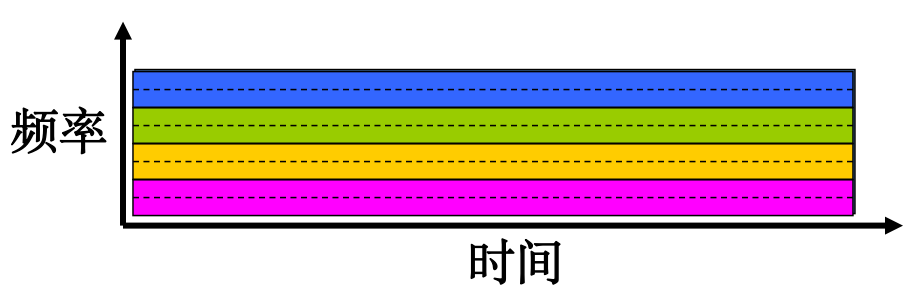
\includegraphics[width=0.74\textwidth]{ch02-fdm.png}
 \caption{FDM把同一时间的信号安排在不同频率带内。来源：\texttt{Chapter2-物理层.pdf}，PDF第36页（显示页36），局部截取。}
 \label{fig:fdm}
\end{figure}
图中纵轴为频率、横轴为时间，四条水平色带表示四个用户分别占用的频率范围；每条带在整个时间方向持续存在。

\textbf{时分复用（TDM）}把时间划成重复出现的TDM帧，每帧再分固定时隙，各用户在各自时隙使用该通路。图\ref{fig:tdm}中的A、B、C、D不是四个不同频带，而是在同一频带上依次获得发送时间；A的时隙每帧重复一次。

\begin{figure}[H]
 \centering
 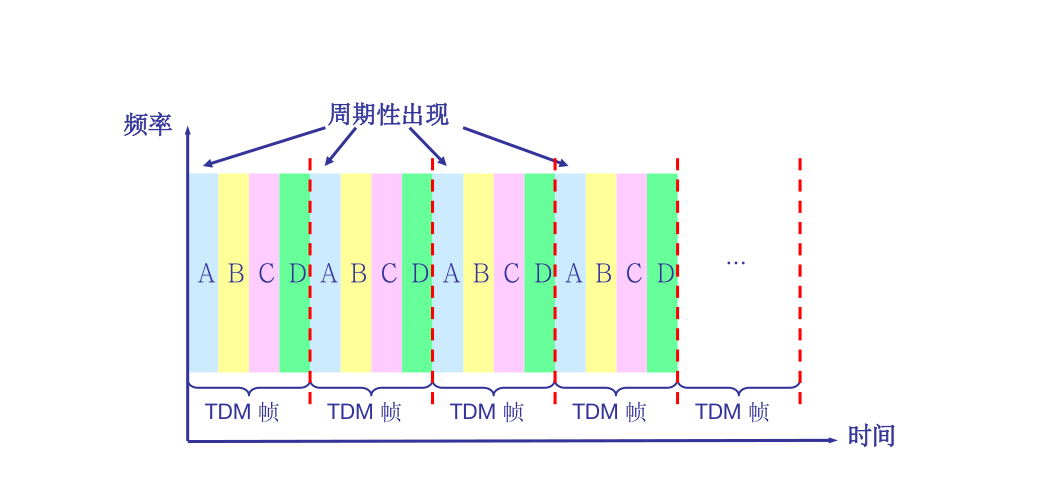
\includegraphics[width=0.82\textwidth]{ch02-tdm.png}
 \caption{TDM帧中的固定时隙周期性重复。来源：\texttt{Chapter2-物理层.pdf}，PDF第38页（显示页38），局部截取。}
 \label{fig:tdm}
\end{figure}

课件图中一个TDM帧包含A、B、C、D四个固定时隙，后续帧按同样次序重复；同一用户的时隙周期性出现。各用户在不同时间使用相同频带。这里的TDM帧是信道时间的周期单位，不是数据链路层的数据帧。固定分配的时隙即使暂时没有数据，也可能闲置。

\textbf{波分复用（WDM）}用不同光波长在同一根光纤上传输。波长与频率对应，故课件把WDM理解为光的频分复用。课件第40页中8路各2.5 Gb/s合成20 Gb/s，是各路数据率相加的例子；前提是共享光纤系统能容纳这些波长通道，并忽略额外开销。

\begin{figure}[H]
 \centering
 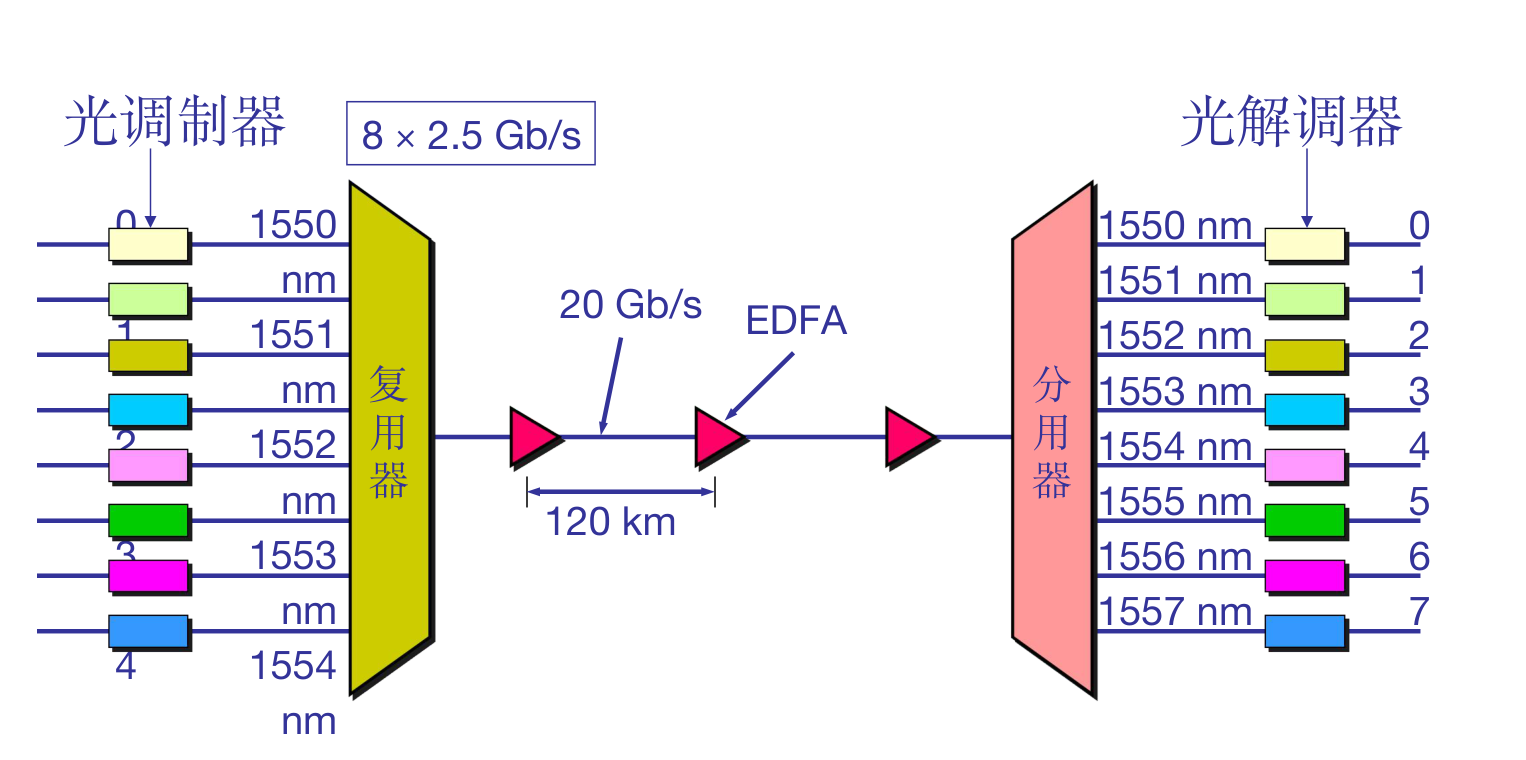
\includegraphics[width=0.92\textwidth]{ch02-wdm.png}
 \caption{WDM用不同波长承载多路光信号，并在接收端分离。来源：\texttt{Chapter2-物理层.pdf}，PDF第40页（显示页40），局部截取。}
 \label{fig:wdm}
\end{figure}
图中8个通道分别使用1550--1557 nm波长，复用器把各波长的光信号合到一根光纤，接收端分用器再分开；EDFA为掺铒光纤放大器，课件标注光纤段约120 km。计算总数据率时，$8\times2.5=20$ Gb/s。
\annotationarea[4]

\subsection{CDM：靠正交码片分离同频用户}
\textbf{码分复用（CDM）}给用户分配不同码片序列，让用户在同一频带、同一时间发送。一个信息比特展开成$m$个\textbf{码片}；每码片在理想数学模型中取$+1$或$-1$。用$d_i=+1$表示信息比特1，用$d_i=-1$表示信息比特0；未发送时记$d_i=0$。

用户$i$的码片向量记为$S_i$。发送1时发送$S_i$，发送0时发送$-S_i$，也就是把每个码片正负反转。接收端看到各用户信号的叠加：
\[
 P=\sum_i d_iS_i.
\]
这个式子只要求同一位置相加。两用户在某位置都发送$+1$，叠加值就为2；一正一负则为0，所以合成信号不必仍只有$\pm1$。

\textbf{内积是什么？} 两个等长向量的内积就是对应元素相乘，再将结果相加，例如$(1,-1)\cdot(1,1)=1-1=0$。两个码片序列内积为0，称它们\textbf{正交}。课件要求不同用户的码片码相互正交，而同一码的自内积为$m$，因此可用
\[
 d_i=\frac{S_i\cdot P}{m}
\]
恢复用户$i$的数据：别人的码与$S_i$点乘为0被消去，自己的码产生$m$倍，除以$m$回到原值。

\textbf{课件示例码片序列（PDF第41页／显示页41）：} 课件给出的一个用户码为
\[
S=(-1,-1,-1,+1,+1,-1,+1,+1).
\]
若码片长度为$m$，同一用户码的自内积为$S_i\cdot S_i=m$；不同用户码两两正交，即$i\ne j$时$S_i\cdot S_j=0$。

\textbf{课件编解码例题（PDF第43--44页／显示页43--44）：} 图\ref{fig:cdm-example}给出用户1、用户2的码片与两个时隙的数据。按图中码片顺序读取，
\[
 S_1=(1,1,1,-1,1,-1,-1,-1),\qquad
 S_2=(1,-1,1,1,1,1,-1,1),\qquad m=8.
\]
为避免下标混淆，记$b_{u,t}$为用户$u$在时隙$t$发送的数据值；$+1$表示比特1，$-1$表示比特0。课件图中用户1在时隙1发送0、时隙0发送1，用户2在两个时隙都发送1，即$b_{1,1}=-1$、$b_{1,0}=+1$、$b_{2,1}=+1$、$b_{2,0}=+1$。
先核对正交：
\[
S_1\cdot S_2=1-1+1-1+1-1+1-1=0.
\]
时隙1的信道输出是两个编码序列逐项相加：
\[
P_1=b_{1,1}S_1+b_{2,1}S_2=-S_1+S_2=(0,-2,0,2,0,2,0,2).
\]
时隙0中两个用户都发送1，因此
\[
P_0=b_{1,0}S_1+b_{2,0}S_2=S_1+S_2=(2,0,2,0,2,0,-2,0).
\]
对每个接收用户，用$\hat b_{u,t}=(S_u\cdot P_t)/8$解码。时隙1：$S_1\cdot P_1=-8$，故用户1数据为$-1$（比特0）；$S_2\cdot P_1=8$，故用户2数据为$+1$（比特1）。时隙0：$S_1\cdot P_0=8$且$S_2\cdot P_0=8$，两用户均解得$+1$（比特1）。

\begin{figure}[H]
 \centering
 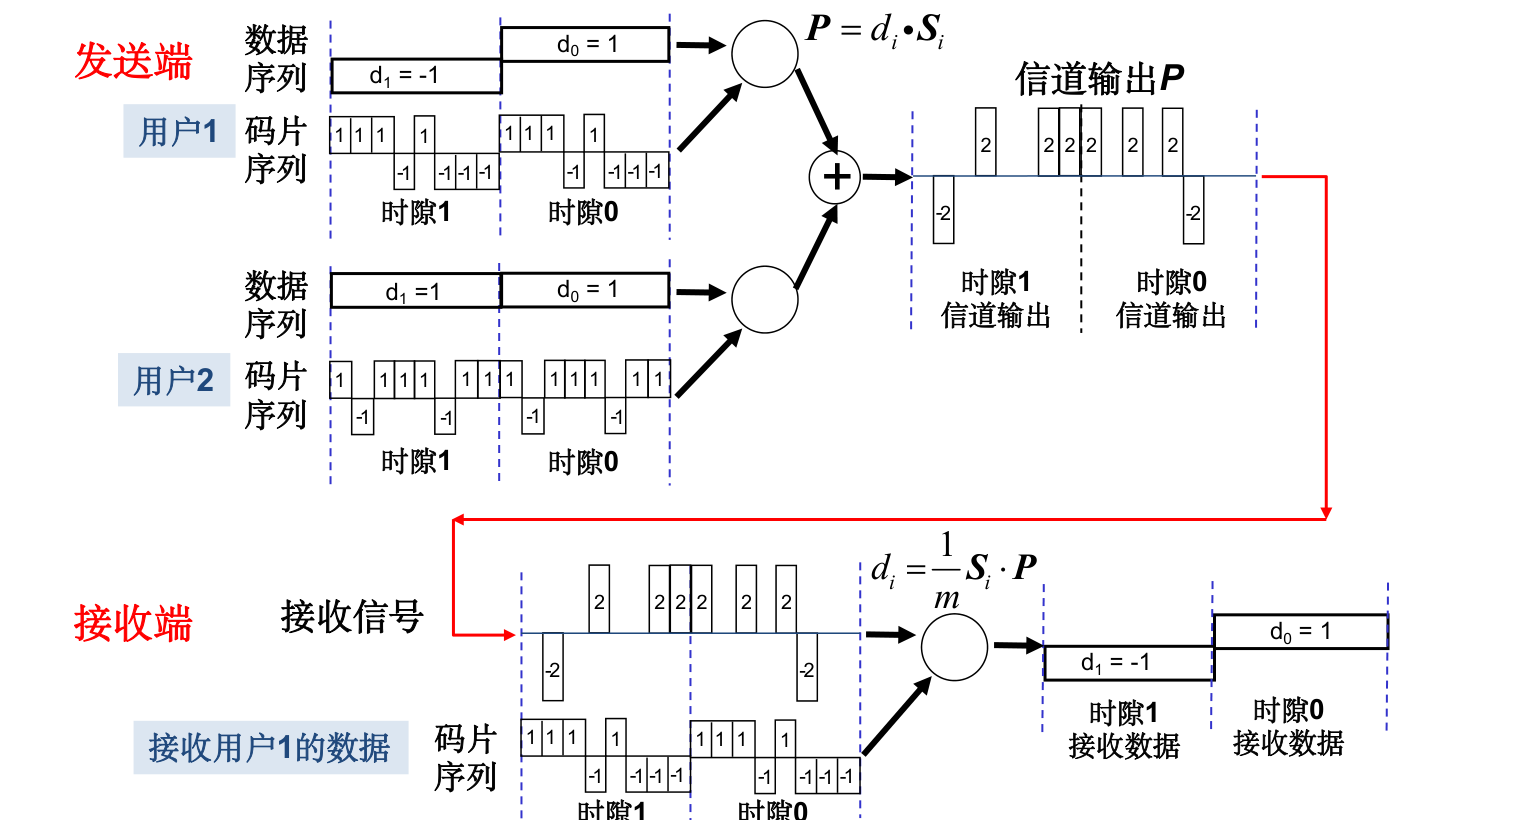
\includegraphics[width=0.96\textwidth]{ch02-cdm-example.png}
 \caption{课件CDM双用户双时隙编解码例。来源：\texttt{Chapter2-物理层.pdf}，PDF第44页（显示页44），局部截取。}
 \label{fig:cdm-example}
\end{figure}
\textbf{适用条件与易错点。} 以上是码片对齐、理想正交、按相同幅度归一且无噪声的模型；实际接收结果会受到噪声、不同功率、时延和多径影响。理想模型中的解码值0表示该用户未发送，\textbf{不表示它发送了信息比特0}。码片也不是原始信息比特：每信息比特展开$m$码片时，码片速率为信息比特率的$m$倍。

\begin{quote}\small 来源：课件PDF第32--44页（显示页32--44）；FDM图取第36页，TDM图取第38页，WDM图取第40页，CDM例图取第44页，均为局部截取。教材第2章没有按这一结构集中讲复用，本节定义、编码与解码以课件为直接依据。\end{quote}
\annotationarea[4]

\section{基带传输}\label{sec:baseband}
\subsection{直接传送基带信号与线路编码}
\textbf{基带信号}是未经搬移到载波频带的原始信号，往往含较多低频甚至直流成分。\textbf{基带传输}是在信道中直接传输基带信号；数字基带传输先把比特映射为适合线路的电平或跳变，再直接发送。这里的\textbf{线路编码}规定“0和1在波形上怎样表现”，不等同于PCM的样本数字化，也不等同于压缩文件。

基带通常适合具有低通特性的有线通路；信号在途中可能衰减、畸变或受噪声影响。选择码型时既要让接收方区分0、1，还要考虑同步信息、直流分量及占用带宽。以下规则按课件约定，遇到采用相反0/1定义的题目应先读其约定。
\annotationarea[4]

\subsection{NRZ、RZ、差分码与AMI}
\textbf{不归零码（NRZ）}在一个比特区间内保持相应电平，区间中途不强制回零。课件的\emph{单极NRZ}用$+E$表示1、0电平表示0；\emph{双极NRZ}用正负电平表示两种比特。这里单极/双极描述使用的电平，归零/不归零描述区间内是否回零，二者是不同分类维度。

\begin{figure}[H]
 \centering
 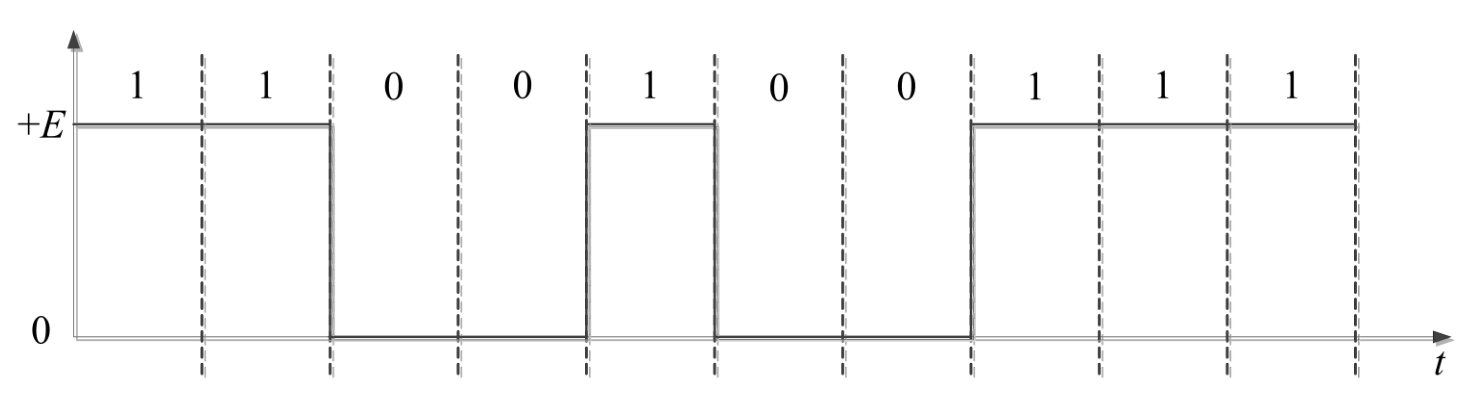
\includegraphics[width=0.85\textwidth]{ch02-nrz-wave.png}
 \caption{单极NRZ：连续相同比特可没有边界跳变。来源：\texttt{Chapter2-物理层.pdf}，PDF第48页（显示页48），波形局部截取。}
 \label{fig:nrz-wave}
\end{figure}

图\ref{fig:nrz-wave}中顶部数字给出每个比特的值，虚线划分区间。连续两个1保持同一电平，连续三个0也是如此；若没有额外时序线索，只观察这段平直线不能知道它跨了几个比特。NRZ本身不保证自同步，实际系统需要另设同步机制。

课件第49页的双极NRZ用$+E$和$-E$分别表示两种比特。课件图的共同输入序列为$1100100111$：单极NRZ输出电平依次为$+E,+E,0,0,+E,0,0,+E,+E,+E$；双极NRZ按“1为$+E$、0为$-E$”的图示约定，输出为$+E,+E,-E,-E,+E,-E,-E,+E,+E,+E$。

\textbf{归零码（RZ）}在每比特的部分时段保持相应非零脉冲，随后回到零。课件单极RZ用正脉冲表示1、全程零表示0；双极RZ用正/负脉冲分别表示两种比特并都回零。占空比是一个区间内非零脉冲占据的时间比例，可写为$D=T_{\mathrm{nz}}/T_b$，其中$T_{\mathrm{nz}}$为非零脉冲时长、$T_b$为一个码元周期。图\ref{fig:rz-wave}中1的脉冲持续$T_b/2$，所以占空比为50\%。

\begin{figure}[H]
 \centering
 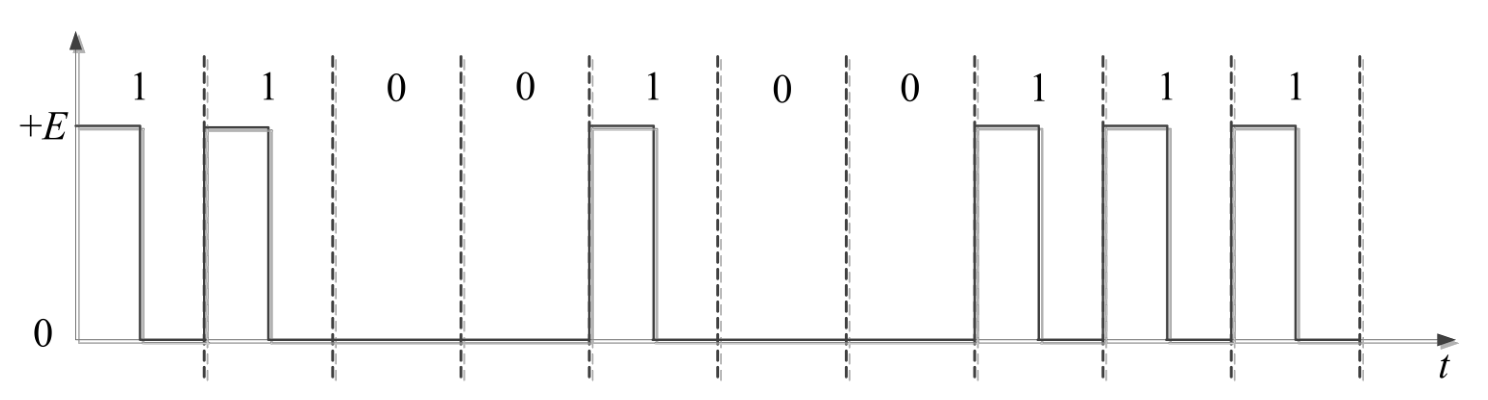
\includegraphics[width=0.85\textwidth]{ch02-rz-wave.png}
 \caption{单极RZ：1的脉冲中途归零，0仍为零电平。来源：\texttt{Chapter2-物理层.pdf}，PDF第50页（显示页50），波形局部截取。}
 \label{fig:rz-wave}
\end{figure}

回零增加电平变化，通常增加对频率带宽的要求。\textbf{单极RZ遇长串0仍没有跳变，不能保证所有比特序列都有同步线索}；双极RZ每比特有非零脉冲并回零，提供的时序线索不同。不能只看到RZ名称就断言“一定自同步”。

课件第51页的双极RZ在比特区间前半段用$+E$表示1、$-E$表示0，后半段都回到零；它与双极NRZ的区别是码元中途是否回零。

\textbf{差分码（相对码）}用相邻码元之间是否发生电平变化表达信息。课件第52页约定“发生跳变表示1、不跳变表示0”。课件波形输入为$1100100111$；以图示的首个电平$+E$为初始状态，首位之后每遇到1就在$0$与$+E$之间翻转，遇到0就保持，输出电平依次为$+E,0,0,0,+E,+E,+E,0,+E,0$。教材介绍的NRZI采用“起始跳变表示0、不变表示1”的常见另一约定。遇到具体题目要按题目给出的0/1约定和初始状态编码。
\annotationarea[4]

\textbf{AMI（Alternative Mark Inversion，信号交替反转码）}把0编码成零电平，依次出现的1交替编码成$+E$、$-E$。课件第53页图中AMI传输码元序列为$+1,0,0,0,0,-1,0,0,0,0,+1,-1,0,0,0,0,+1,-1$；按“0为零电平、正负脉冲都代表信息位1”解码，信息位为$100001000011000011$。长串0仍没有跳变。
\annotationarea[4]

\subsection{Manchester与差分Manchester：每位都有同步跳变}
\textbf{Manchester编码}把一个比特时间分为两半，中间必须跳变。按课件第54页：高到低表示1，低到高表示0。中点的跳变既标示时序，又用方向表示数据；比特边界是否跳变由相邻数据决定，不能把边界跳变误当成中点规则。

\textbf{差分Manchester编码}也在每比特中点跳变，但中点只用于同步；数据由比特\emph{开始处}是否跳变表示。按课件第55页：起始跳变表示0，起始不跳变表示1。它与课件第52页的普通差分码相比，多了每比特中点的固定跳变，规则也不同。

\begin{figure}[H]
 \centering
 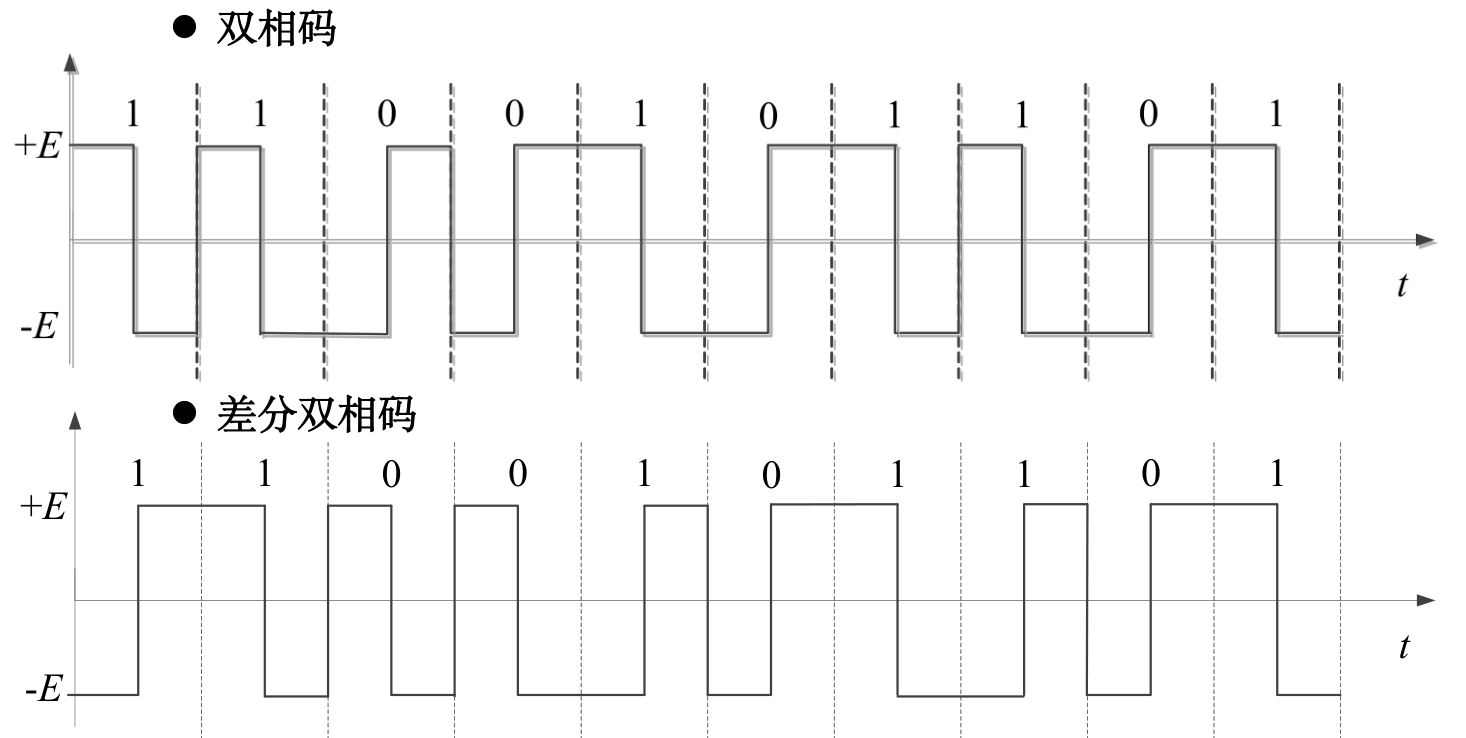
\includegraphics[width=0.93\textwidth]{ch02-line-codes.png}
 \caption{上：Manchester；下：差分Manchester。来源：\texttt{Chapter2-物理层.pdf}，PDF第56页（显示页56），波形局部截取。}
 \label{fig:line-codes}
\end{figure}

\textbf{读图方法。} 先用顶部0/1及竖线定位每比特区间，再看区间中点跳变；对下图还需看每比特起点，第一位的起点要依已知初始参考电平判断。上下图的中点跳变都服务同步，但只有上图按中点方向读数据。

\textbf{课件例题（PDF第56页／显示页56）：} 输入比特为$1100101101$。按课件给定的Manchester约定逐位编码：
\begin{center}
\begin{tabular}{lcccccccccc}
\toprule
输入比特 & 1 & 1 & 0 & 0 & 1 & 0 & 1 & 1 & 0 & 1\\
\midrule
Manchester & HL & HL & LH & LH & HL & LH & HL & HL & LH & HL\\
差分Manchester & LH & HL & HL & HL & LH & LH & HL & LH & LH & HL\\
\bottomrule
\end{tabular}
\end{center}
表中H、L分别表示高、低电平；例如HL表示一个比特前半周期为高、后半周期为低。Manchester每个比特中点都跳变，H到L表示1、L到H表示0。差分Manchester每个中点也跳变，中点只用于同步；比特起点跳变表示0、不跳变表示1。按课件图示，首位开始前的参考电平为L；逐位依据前一位终点和当前比特计算，得到表中的差分Manchester波形。初始参考电平不同会使整条波形整体反相，但相对变化规则不变。
\annotationarea[4]

两种编码都通过固定中点跳变提高时钟恢复能力，代价是同一比特率下更多电平变化、通常需要更宽带宽。课件称用两个脉冲编码一比特；这不表示有效数据比特率被算作原来的两倍。10 Mb/s传统以太网采用Manchester，是后文Ethernet的基础。
\annotationarea[4]

\subsection{nBmB：用冗余码组改善线路特性}
\textbf{nBmB编码}把$n$位数据映射为$m$位新码组，其中$m>n$。$2^n$种数据组合从$2^m$个码组中选择合适表示，使线路上更容易出现需要的跳变等特性。冗余还可留出控制、保留或无效码组；出现无效组可提示差错，但不是所有差错都能检出。

课件以\textbf{4B5B}为例：4位数据有16种组合，5位线路码有32种组合，从中选16种代表数据，其余可承担其他用途或禁用。\textbf{课件表述修正：} 第57页将余下16种一概称作“禁用码”，实际应区分控制码、保留码和无效码，不能把任意非数据码都认作传输出错。

\textbf{自拟计算：} 输入数据率100 Mb/s，经4B5B映射且不计其他开销，线路码比特率为$100\times5/4=125$ Mb/s；数据占线路码的$4/5=80\%$，线路位数比输入增加25\%。4B5B是分组映射，常还需配合具体线路波形编码；它本身不是“用五种电压发送四比特”。课件列出的100BASE-TX/FX是使用该映射的实例，不推广为所有快速以太网都相同。
\annotationarea[4]

\begin{quote}\small 来源：课件PDF第45--57页（显示页45--57）；教材§2.1.3，PDF第44--45页／印刷第33--34页。本节显式区分课件差分码与教材NRZI的0/1约定，并补全单极RZ长0与4B5B余码的边界。\end{quote}
\annotationarea[4]

\section{频带传输}\label{sec:passband}
\subsection{载波、幅度、频率与相位}
许多信道适合通过一段离开零频的频带，而不能直接通过所需基带波形。\textbf{频带传输}让基带数据控制载波的某些参数，把信息放到适合信道的频带上；接收端再作解调。频带传输不是“发送更多频率就一定更快”，而是适配信道的传输技术。

载波常写成
\[
 s(t)=A\cos(2\pi ft+\phi).
\]
$A$是振幅，表示波形离中心线的最大幅度；$f$是频率（Hz），表示每秒振荡多少周期；$\phi$是相位，决定某时刻处于周期中的哪一位置。一个周期为$2\pi$弧度，$\pi$是半周期、$\pi/2$是四分之一周期。\textbf{学习补充：} 相位差$\pi$的两条同频同幅余弦波，在同一时刻的取值符号相反；相位差不是频率不同。

课件把模拟基带控制载波称模拟调制，把数字基带控制载波称数字调制。本节集中学习后者。数字调制中的载波仍是连续波形；比特体现在对载波状态的有限种选择中。
\annotationarea[4]

\subsection{二进制调制：每码元两种状态}
\textbf{2ASK（幅移键控）}用两种振幅表示0和1。课件的开关键控示例以有载波表示1、无载波表示0；图\ref{fig:ask-wave}从上到下是数字基带、未调制载波、输出波形。基带为0时输出消失，基带为1时出现振荡。

\begin{figure}[H]
 \centering
 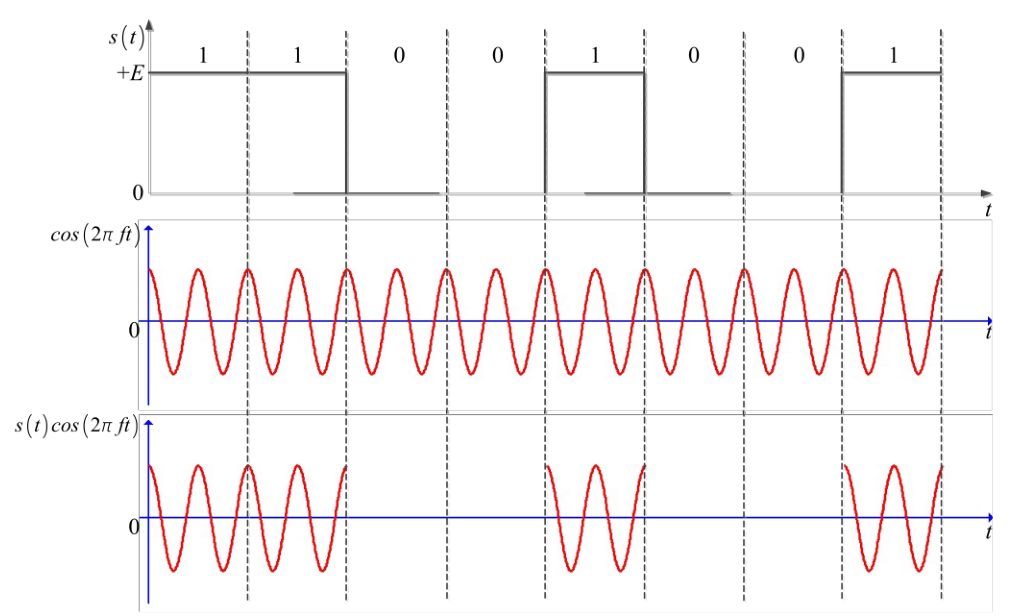
\includegraphics[width=0.69\textwidth]{ch02-ask-wave.png}
 \caption{2ASK通过是否保留载波幅度表达比特。来源：\texttt{Chapter2-物理层.pdf}，PDF第61页（显示页61），波形局部截取。}
 \label{fig:ask-wave}
\end{figure}
课件例图的输入为$11001001$，所以2ASK输出依次为“有载波、有载波、无载波、无载波、有载波、无载波、无载波、有载波”。这里用有无载波表示两种状态。课件的表达式为$y(t)=s(t)\cos(2\pi ft)$，其中$s(t)$是单极数字基带信号，$f$为载波频率；基带为0时幅度为0，基带为1时保留载波。
\annotationarea[4]

\textbf{2FSK（频移键控）}用两个不同频率$f_1$、$f_2$表示0、1，课件第62页约定0用$f_1$、1用$f_2$。图\ref{fig:fsk-wave}中不同码元区间的振荡疏密不同，疏密反映频率，而不只是幅度变化。

\begin{figure}[H]
 \centering
 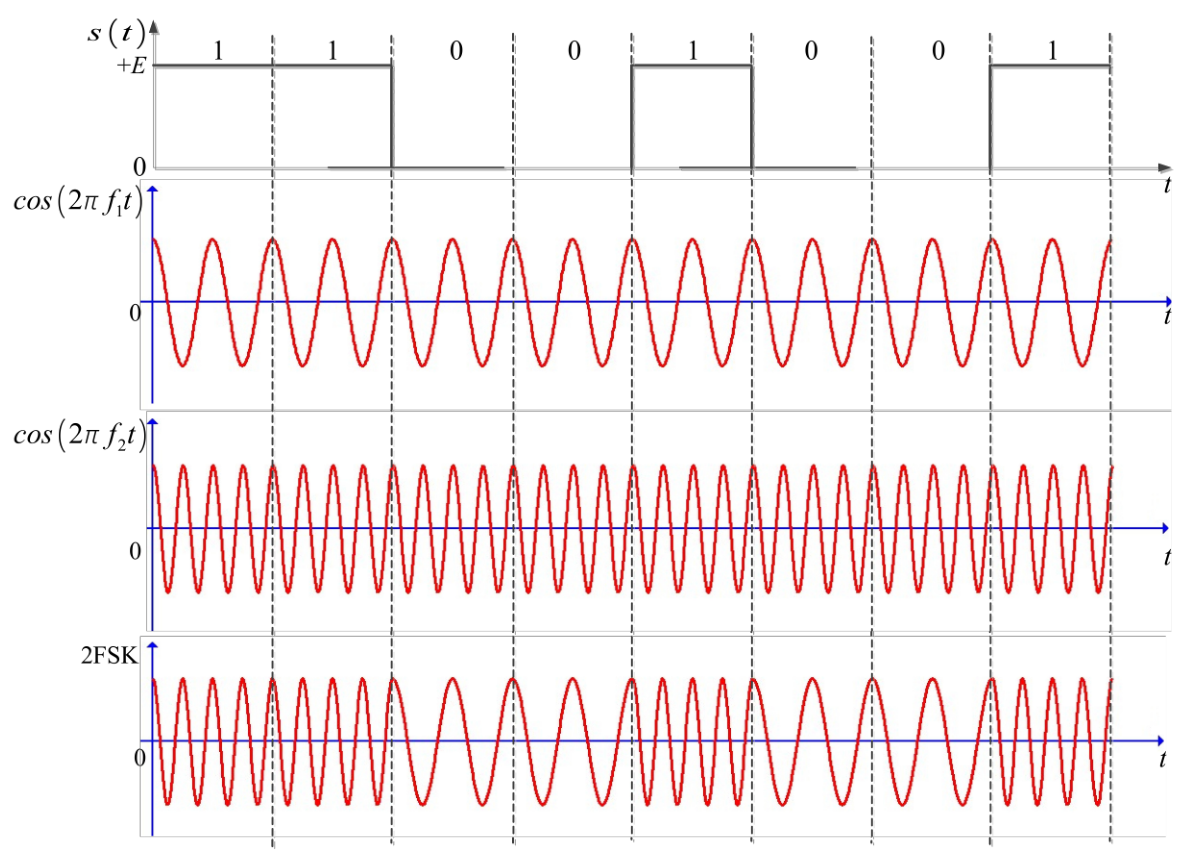
\includegraphics[width=0.69\textwidth]{ch02-fsk-wave.png}
 \caption{2FSK在两种载波频率中选择。来源：\texttt{Chapter2-物理层.pdf}，PDF第63页（显示页63），波形局部截取。}
 \label{fig:fsk-wave}
\end{figure}
课件例图输入仍为$11001001$；逐位替换为载波频率后，输出频率顺序为$f_2,f_2,f_1,f_1,f_2,f_1,f_1,f_2$。在第$n$个码元区间，课件约定$y(t)=\cos(2\pi f_1t)$表示0、$y(t)=\cos(2\pi f_2t)$表示1；$f_1$、$f_2$是两种不同载波频率。
\annotationarea[4]

\textbf{2PSK（相移键控）}用两种绝对相位表示比特，课件第64页以$\phi_0$表示0、$\phi_0+\pi$表示1。一个码元内可写为$y(t)=\cos(2\pi ft+\phi_n)$，其中$\phi_n=\phi_0$对应0、$\phi_n=\phi_0+\pi$对应1。绝对相位的判断需要接收方有相位参考。图\ref{fig:psk-wave}采用$\phi_0=-\pi/2$作示例，重点看相位对应关系，不必把该初始值背成所有系统的固定值。

\begin{figure}[H]
 \centering
 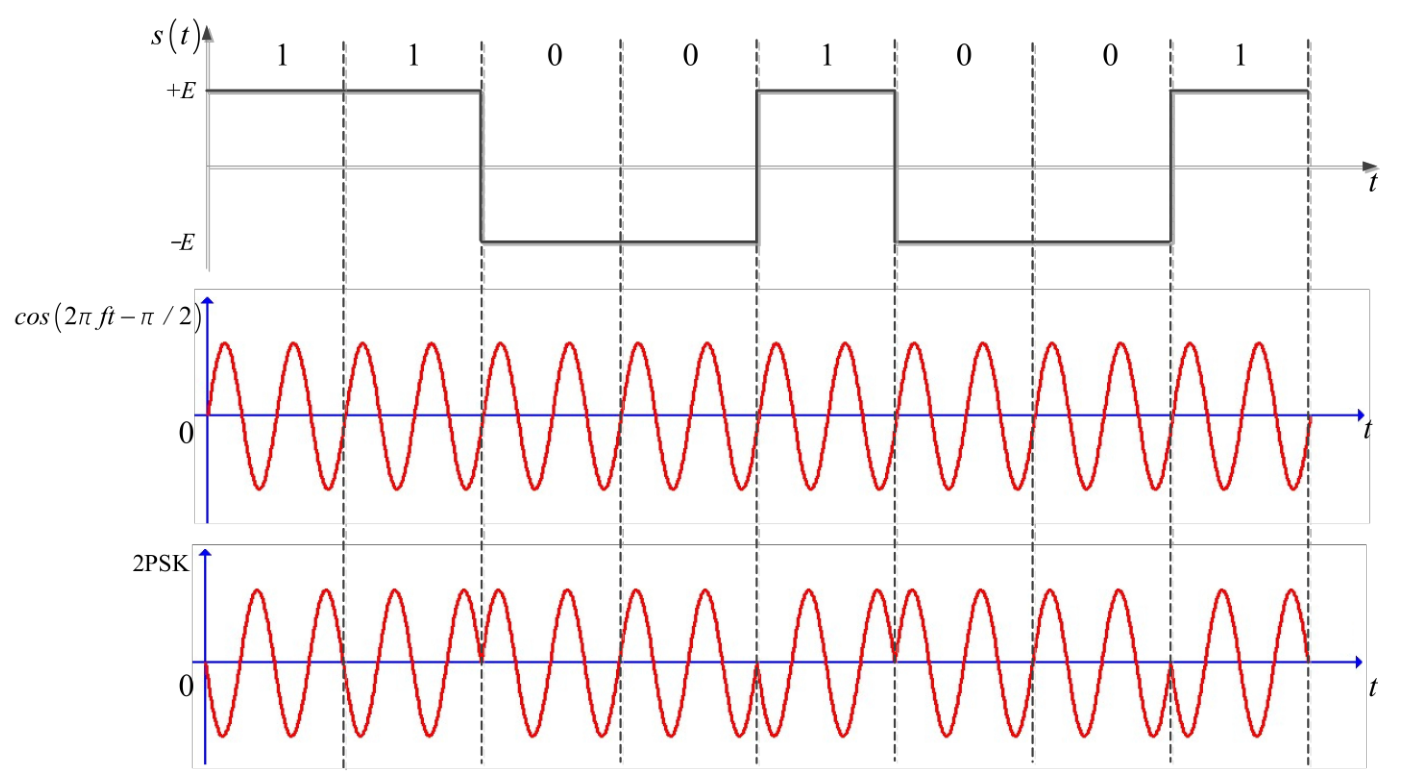
\includegraphics[width=0.83\textwidth]{ch02-psk-wave.png}
 \caption{2PSK以相差半周期的两种相位表达0与1。来源：\texttt{Chapter2-物理层.pdf}，PDF第65页（显示页65），波形局部截取。}
 \label{fig:psk-wave}
\end{figure}
\textbf{课件例题（PDF第65页／显示页65）：} 输入$11001001$，按“0取$\phi_0$、1取$\phi_0+\pi$”逐位查表，得到
\[
(\phi_0+\pi,\phi_0+\pi,\phi_0,\phi_0,\phi_0+\pi,\phi_0,\phi_0,\phi_0+\pi).
\]
代入课件的$\phi_0=-\pi/2$，绝对相位为
\[
(\pi/2,\pi/2,-\pi/2,-\pi/2,\pi/2,-\pi/2,-\pi/2,\pi/2).
\]
\annotationarea[4]

\textbf{2DPSK（二进制差分相移键控）}用相邻码元载波的相对相位变化表示信息。课件第66页约定：比特0使相位不变，记$\Delta\phi_n=0$；比特1使相位改变$\pi$，记$\Delta\phi_n=\pi$。因此第$n$个码元相位为前一码元相位加本位相位变化，可写成$y(t)=\cos(2\pi ft+\phi_{n-1}+\Delta\phi_n)$。接收端比较相邻码元相位即可解码，不必判断一个绝对相位基准。

\begin{figure}[H]
 \centering
 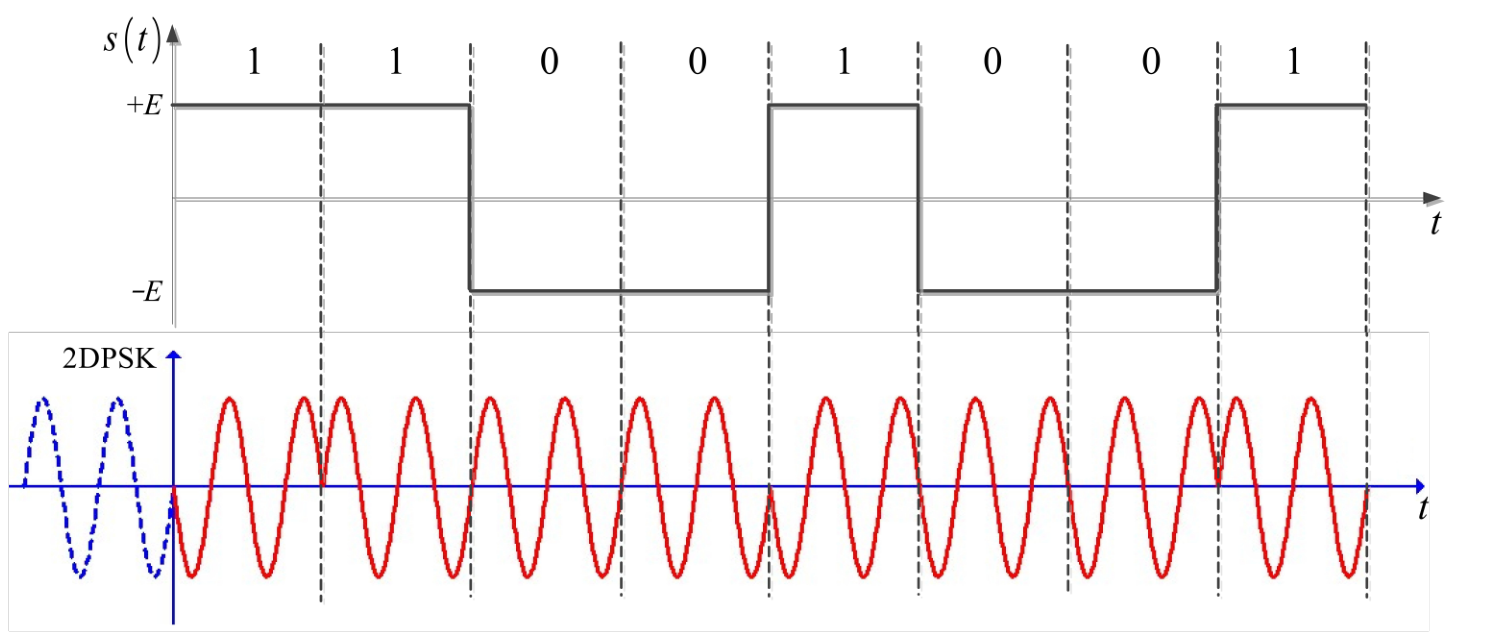
\includegraphics[width=0.92\textwidth]{ch02-dpsk-wave.png}
 \caption[2DPSK波形示意]{2DPSK例图中的虚线表示前一码元信号或初始参考载波。来源：Chapter2-物理层.pdf，PDF第67页（显示页67），局部截取。}
 \label{fig:dpsk-wave}
\end{figure}
图\ref{fig:dpsk-wave}中虚线是当前序列之前的参考，红色波形是已调信号；出现反相表示相位差$\pi$，相位连续表示相位差0。\textbf{课件例题（PDF第67页／显示页67）：} 输入$11001001$，以虚线参考相位$\phi_{-1}=0$为起点，依次累计相位变化$\pi,\pi,0,0,\pi,0,0,\pi$，各码元相位为$\pi,0,0,0,\pi,\pi,\pi,0$（模$2\pi$）。
\annotationarea[4]

\textbf{课件中的二进制调制性能比较（PDF第68页／显示页68）：}
\begin{center}
\small
\begin{tabularx}{0.97\textwidth}{l X}
\toprule
比较项目 & 课件给出的结论\\
\midrule
频带利用率 & 2ASK、2PSK、2DPSK相同；2FSK最低\\
误码率 & 在相同信噪比下，2PSK最低、2ASK最高；课件给出的抗噪声性能顺序为2PSK优于2FSK、2FSK优于2ASK\\
对信道特性变化的敏感性 & 2ASK较敏感；2FSK和2PSK较不敏感\\
\bottomrule
\end{tabularx}
\end{center}
这是课件采用的典型比较结论；具体系统比较还要核对信噪比定义、接收方式和其他条件。
\annotationarea[4]

\subsection{多进制与QAM：怎样阅读星座图}
二进制调制每码元只有两种状态，多进制调制让每码元选择更多状态。仍使用2.2节的关系
\[
 R_b=R_B\log_2M.
\]
\textbf{自拟例：} 1200 Baud、16种状态时，$R_b=1200\times4=4800$ b/s。若保持波特率不变而用64种状态，每码元6 bit，比特率变为7200 b/s；接收方要在同样时间里作更细致的状态区分。
\annotationarea[4]
课件同时指出，多进制数字调制需要更高的信噪比；发送端可增大发射信号功率以便接收端区分更多状态。
\annotationarea[4]

\textbf{正交幅度调制（QAM，Quadrature Amplitude Modulation）}又称幅值相位联合键控（APK），组合两条同频、相差$90^\circ$的载波。课件指出QAM频带利用率高、设备较简单，并可自适应调整调制速率。在课件记号下，一码元区间内的信号为
\[
 y(t)=A_n\cos(2\pi ft)+B_n\sin(2\pi ft),
\]
其中$A_n$、$B_n$分别控制同相I支路与正交Q支路的幅度，可取带正负号的离散值。课件也把合成信号写成$y(t)=s_n\cos(2\pi ft+\phi_n)$，其中$A_n=s_n\cos\phi_n$、$B_n=-s_n\sin\phi_n$；$s_n$和$\phi_n$分别表示该码元合成载波的幅度与相位。这里“正交”指两种基函数在一个合适码元区间上的内积为0，因此接收端可分别估计I、Q分量。

\textbf{星座图怎样看？} 横轴I和纵轴Q分别记两支路幅度，每个点$(A_n,B_n)$代表一种合成信号状态。到原点的距离与合成幅度对应，围绕原点的方向与合成相位对应（正负相位约定依系统）。方形16QAM每支路有4个可选幅度，组合为$4\times4=16$个点，每点对应4 bit；方形64QAM每支路有8个幅度，共64点，每点6 bit。接收方估计I/Q分量并判定最接近哪个合法点，然后恢复该点对应的比特组合。

\begin{figure}[H]
 \centering
 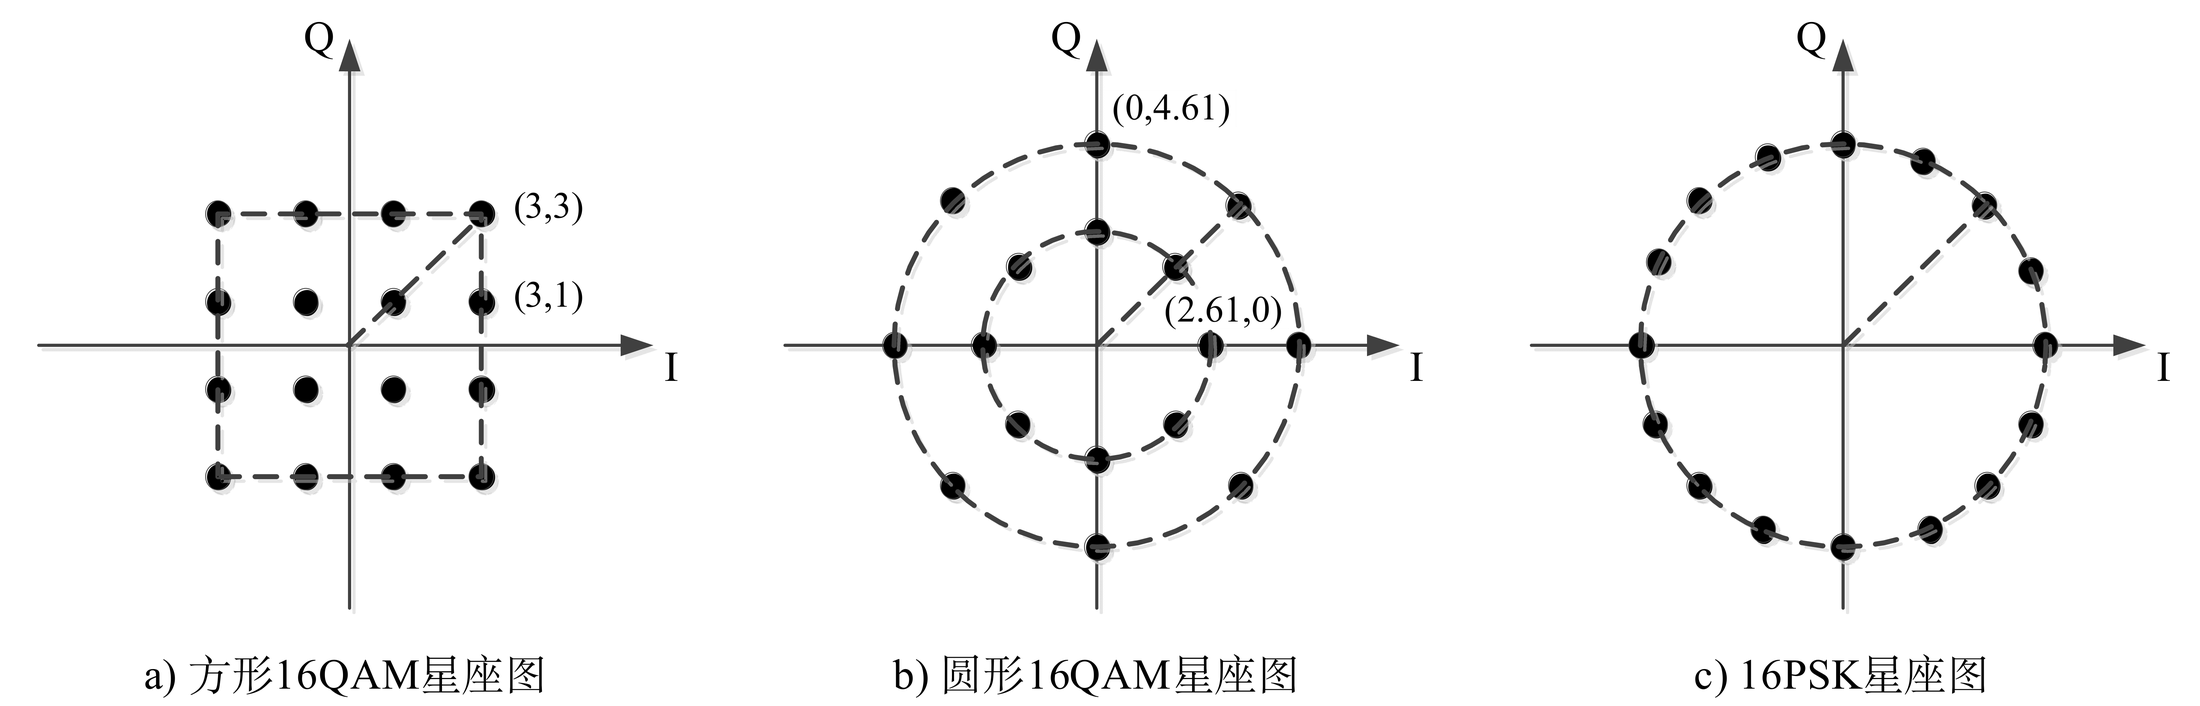
\includegraphics[width=0.93\textwidth]{ch02-qam.png}
 \caption{左：方形16QAM；中：圆形16QAM；右：16PSK对照图。来源：\texttt{Chapter2-物理层.pdf}，PDF第71页（显示页71），星座图局部截取。右图各点在同一圆周上，区别主要在相位，不应称为QAM图。}
 \label{fig:qam-constellation}
\end{figure}

课件第30页题目说“4相位、每相位4幅度”，直接按题设得到16状态；不要把它误当作方形16QAM必定只有4个极角。\textbf{学习补充：} 在同样平均发送功率下，星座点越多通常越拥挤，噪声更容易使接收点跨入邻点的判决区域，往往要求更高信噪比。QAM可提高频带利用率，但“QAM抗噪能力强”不能脱离阶数、能量和接收条件作绝对比较。

\textbf{易错点。} 编码是确定数字表示/线路码的规则；数字调制是控制载波状态。本章不同处理可连续使用，例如先把语音PCM数字化，再做冗余编码，再用QAM发送。Hz是频带宽度，Baud是码元数，bit/s是信息比特数；三种单位仍须分别保留。

\begin{quote}\small 来源：课件PDF第58--71页（显示页58--71）；教材§2.1.3，PDF第45--46页／印刷第34--35页。课件典型性能比较的条件在正文中显式提示，避免把示例结论推广为所有实现的排名。\end{quote}
\annotationarea[4]

\section{物理层设备}
\subsection{中继器：再生信号}
信号经过较长线路会减弱、变形。\textbf{中继器（Repeater）}按接收到的信号恢复应有的比特时序和波形，再向后发送，扩大可覆盖距离。图\ref{fig:repeater-regeneration}左侧是衰减失真的脉冲，右侧是再生后的规整脉冲。它的原理是再生，不能只理解为把电压乘一个系数；简单放大也会放大噪声。

\begin{figure}[H]
 \centering
 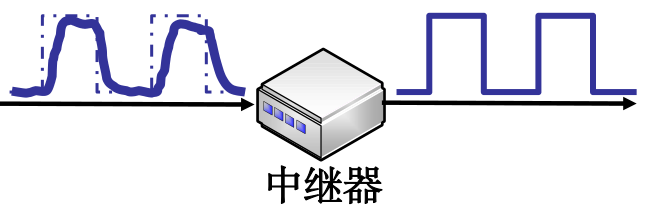
\includegraphics[width=0.68\textwidth]{ch02-repeater-regeneration.png}
 \caption{中继器将失真信号再生为规定波形。来源：\texttt{Chapter2-物理层.pdf}，PDF第73页（显示页73），局部截取。}
 \label{fig:repeater-regeneration}
\end{figure}

\textbf{适用边界。} 中继器不理解MAC地址或帧内容，也不完成不同数据链路协议的转换。如果输入信号已被误判，再生只会把误判后的比特继续发出，不能当成可靠纠错器。中继器数量也受相应网络标准和传播时延限制，不能无限串联扩展一个网络。
\annotationarea[4]

\subsection{集线器：多端口中继器}
\textbf{集线器（Hub）}相当于多端口中继器：一个端口收到的信号会再生并转发到其他端口，课件称各端口在内部物理连通。它不查找目的地址，不决定某个帧应只去哪个端口，也不学习地址表。使用Hub连接多台主机，线缆在物理上呈星形，通信逻辑仍共享同一通路。

\textbf{参考书补充：} Hub的各端口属于同一\emph{冲突域}，即多个发送端可能同时发送并发生冲突的范围。它按信号扩散方式转发，不按目的地址筛选端口，因此也不能分割广播域。课件第73页只强调Hub是多端口中继器、所有端口内部物理连通，并列出10BASE-T和100BASE-T以太网应用；冲突域等概念由参考书用于进一步解释。
\annotationarea[4]

\begin{quote}\small 来源：课件PDF第72--74页（显示页72--74）；教材§2.3--§2.4，PDF第57--60页／印刷第46--49页。\end{quote}

\subsection*{本章回顾}
物理层在物理介质上实现比特流传输。数据通信先将数据变成适合信道传送的信号；信道类型和容量限制可达到的传输速率。物理介质分导引型与非导引型；奈奎斯特公式讨论理想无噪声、带宽受限的容量，香农公式讨论有噪声信道的容量上限。信道共享可用FDM、TDM、WDM和CDM。基带传输直接发送基带信号，频带传输通过调制载波适配带通信道。中继器和集线器是课件列出的物理层设备，均以比特再生为基本工作原理。
\annotationarea[4]
